% Options for packages loaded elsewhere
\PassOptionsToPackage{unicode}{hyperref}
\PassOptionsToPackage{hyphens}{url}
%
\documentclass[
]{article}
\usepackage{amsmath,amssymb}
\usepackage{lmodern}
\usepackage{iftex}
\ifPDFTeX
  \usepackage[T1]{fontenc}
  \usepackage[utf8]{inputenc}
  \usepackage{textcomp} % provide euro and other symbols
\else % if luatex or xetex
  \usepackage{unicode-math}
  \defaultfontfeatures{Scale=MatchLowercase}
  \defaultfontfeatures[\rmfamily]{Ligatures=TeX,Scale=1}
\fi
% Use upquote if available, for straight quotes in verbatim environments
\IfFileExists{upquote.sty}{\usepackage{upquote}}{}
\IfFileExists{microtype.sty}{% use microtype if available
  \usepackage[]{microtype}
  \UseMicrotypeSet[protrusion]{basicmath} % disable protrusion for tt fonts
}{}
\makeatletter
\@ifundefined{KOMAClassName}{% if non-KOMA class
  \IfFileExists{parskip.sty}{%
    \usepackage{parskip}
  }{% else
    \setlength{\parindent}{0pt}
    \setlength{\parskip}{6pt plus 2pt minus 1pt}}
}{% if KOMA class
  \KOMAoptions{parskip=half}}
\makeatother
\usepackage{xcolor}
\IfFileExists{xurl.sty}{\usepackage{xurl}}{} % add URL line breaks if available
\IfFileExists{bookmark.sty}{\usepackage{bookmark}}{\usepackage{hyperref}}
\hypersetup{
  pdftitle={Notes: R For Beginners},
  pdfauthor={Wai},
  hidelinks,
  pdfcreator={LaTeX via pandoc}}
\urlstyle{same} % disable monospaced font for URLs
\usepackage[margin=1in]{geometry}
\usepackage{color}
\usepackage{fancyvrb}
\newcommand{\VerbBar}{|}
\newcommand{\VERB}{\Verb[commandchars=\\\{\}]}
\DefineVerbatimEnvironment{Highlighting}{Verbatim}{commandchars=\\\{\}}
% Add ',fontsize=\small' for more characters per line
\usepackage{framed}
\definecolor{shadecolor}{RGB}{248,248,248}
\newenvironment{Shaded}{\begin{snugshade}}{\end{snugshade}}
\newcommand{\AlertTok}[1]{\textcolor[rgb]{0.94,0.16,0.16}{#1}}
\newcommand{\AnnotationTok}[1]{\textcolor[rgb]{0.56,0.35,0.01}{\textbf{\textit{#1}}}}
\newcommand{\AttributeTok}[1]{\textcolor[rgb]{0.77,0.63,0.00}{#1}}
\newcommand{\BaseNTok}[1]{\textcolor[rgb]{0.00,0.00,0.81}{#1}}
\newcommand{\BuiltInTok}[1]{#1}
\newcommand{\CharTok}[1]{\textcolor[rgb]{0.31,0.60,0.02}{#1}}
\newcommand{\CommentTok}[1]{\textcolor[rgb]{0.56,0.35,0.01}{\textit{#1}}}
\newcommand{\CommentVarTok}[1]{\textcolor[rgb]{0.56,0.35,0.01}{\textbf{\textit{#1}}}}
\newcommand{\ConstantTok}[1]{\textcolor[rgb]{0.00,0.00,0.00}{#1}}
\newcommand{\ControlFlowTok}[1]{\textcolor[rgb]{0.13,0.29,0.53}{\textbf{#1}}}
\newcommand{\DataTypeTok}[1]{\textcolor[rgb]{0.13,0.29,0.53}{#1}}
\newcommand{\DecValTok}[1]{\textcolor[rgb]{0.00,0.00,0.81}{#1}}
\newcommand{\DocumentationTok}[1]{\textcolor[rgb]{0.56,0.35,0.01}{\textbf{\textit{#1}}}}
\newcommand{\ErrorTok}[1]{\textcolor[rgb]{0.64,0.00,0.00}{\textbf{#1}}}
\newcommand{\ExtensionTok}[1]{#1}
\newcommand{\FloatTok}[1]{\textcolor[rgb]{0.00,0.00,0.81}{#1}}
\newcommand{\FunctionTok}[1]{\textcolor[rgb]{0.00,0.00,0.00}{#1}}
\newcommand{\ImportTok}[1]{#1}
\newcommand{\InformationTok}[1]{\textcolor[rgb]{0.56,0.35,0.01}{\textbf{\textit{#1}}}}
\newcommand{\KeywordTok}[1]{\textcolor[rgb]{0.13,0.29,0.53}{\textbf{#1}}}
\newcommand{\NormalTok}[1]{#1}
\newcommand{\OperatorTok}[1]{\textcolor[rgb]{0.81,0.36,0.00}{\textbf{#1}}}
\newcommand{\OtherTok}[1]{\textcolor[rgb]{0.56,0.35,0.01}{#1}}
\newcommand{\PreprocessorTok}[1]{\textcolor[rgb]{0.56,0.35,0.01}{\textit{#1}}}
\newcommand{\RegionMarkerTok}[1]{#1}
\newcommand{\SpecialCharTok}[1]{\textcolor[rgb]{0.00,0.00,0.00}{#1}}
\newcommand{\SpecialStringTok}[1]{\textcolor[rgb]{0.31,0.60,0.02}{#1}}
\newcommand{\StringTok}[1]{\textcolor[rgb]{0.31,0.60,0.02}{#1}}
\newcommand{\VariableTok}[1]{\textcolor[rgb]{0.00,0.00,0.00}{#1}}
\newcommand{\VerbatimStringTok}[1]{\textcolor[rgb]{0.31,0.60,0.02}{#1}}
\newcommand{\WarningTok}[1]{\textcolor[rgb]{0.56,0.35,0.01}{\textbf{\textit{#1}}}}
\usepackage{graphicx}
\makeatletter
\def\maxwidth{\ifdim\Gin@nat@width>\linewidth\linewidth\else\Gin@nat@width\fi}
\def\maxheight{\ifdim\Gin@nat@height>\textheight\textheight\else\Gin@nat@height\fi}
\makeatother
% Scale images if necessary, so that they will not overflow the page
% margins by default, and it is still possible to overwrite the defaults
% using explicit options in \includegraphics[width, height, ...]{}
\setkeys{Gin}{width=\maxwidth,height=\maxheight,keepaspectratio}
% Set default figure placement to htbp
\makeatletter
\def\fps@figure{htbp}
\makeatother
\setlength{\emergencystretch}{3em} % prevent overfull lines
\providecommand{\tightlist}{%
  \setlength{\itemsep}{0pt}\setlength{\parskip}{0pt}}
\setcounter{secnumdepth}{-\maxdimen} % remove section numbering
\usepackage{booktabs}
\usepackage{longtable}
\usepackage{array}
\usepackage{multirow}
\usepackage{wrapfig}
\usepackage{float}
\usepackage{colortbl}
\usepackage{pdflscape}
\usepackage{tabu}
\usepackage{threeparttable}
\usepackage{threeparttablex}
\usepackage[normalem]{ulem}
\usepackage{makecell}
\usepackage{xcolor}
\ifLuaTeX
  \usepackage{selnolig}  % disable illegal ligatures
\fi

\title{Notes: R For Beginners}
\author{Wai}
\date{2022-03-12}

\begin{document}
\maketitle

This is a note taking page I used while watching the R For Beginners
Online Training Videos:

\url{https://koliajay.netlify.app/talk/rforbeginners/}

\hypertarget{session-1}{%
\section{Session 1:}\label{session-1}}

\hypertarget{direct-calculation-on-r-r-as-a-big-calc}{%
\subsection{Direct calculation on R (R as a Big
calc)}\label{direct-calculation-on-r-r-as-a-big-calc}}

\begin{Shaded}
\begin{Highlighting}[]
\DecValTok{1}
\end{Highlighting}
\end{Shaded}

\begin{verbatim}
## [1] 1
\end{verbatim}

\begin{Shaded}
\begin{Highlighting}[]
\DecValTok{1} \SpecialCharTok{+} \DecValTok{1}
\end{Highlighting}
\end{Shaded}

\begin{verbatim}
## [1] 2
\end{verbatim}

\begin{Shaded}
\begin{Highlighting}[]
\DecValTok{34}\SpecialCharTok{/}\DecValTok{40}
\end{Highlighting}
\end{Shaded}

\begin{verbatim}
## [1] 0.85
\end{verbatim}

\begin{Shaded}
\begin{Highlighting}[]
\DecValTok{5} \SpecialCharTok{\textless{}} \DecValTok{4}
\end{Highlighting}
\end{Shaded}

\begin{verbatim}
## [1] FALSE
\end{verbatim}

\begin{Shaded}
\begin{Highlighting}[]
\DecValTok{16} \SpecialCharTok{==} \DecValTok{16}
\end{Highlighting}
\end{Shaded}

\begin{verbatim}
## [1] TRUE
\end{verbatim}

\hypertarget{plot-using-r}{%
\subsection{Plot using R}\label{plot-using-r}}

\begin{Shaded}
\begin{Highlighting}[]
\FunctionTok{plot}\NormalTok{(}\DecValTok{1}\SpecialCharTok{:}\DecValTok{100}\NormalTok{)}
\end{Highlighting}
\end{Shaded}

\includegraphics{Walkthrough_notes_files/figure-latex/unnamed-chunk-2-1.pdf}

\hypertarget{r-functions}{%
\subsection{R functions}\label{r-functions}}

A function, in a programming environment, is a set of instructions. A
programmer builds a function to avoid repeating the same task, or reduce
complexity.

\begin{Shaded}
\begin{Highlighting}[]
\CommentTok{\# Rounding}
\FunctionTok{round}\NormalTok{(}\FloatTok{9.1615}\NormalTok{, }\DecValTok{2}\NormalTok{)}
\end{Highlighting}
\end{Shaded}

\begin{verbatim}
## [1] 9.16
\end{verbatim}

\begin{Shaded}
\begin{Highlighting}[]
\CommentTok{\# Square Root}
\FunctionTok{sqrt}\NormalTok{(}\DecValTok{9}\NormalTok{)}
\end{Highlighting}
\end{Shaded}

\begin{verbatim}
## [1] 3
\end{verbatim}

\begin{Shaded}
\begin{Highlighting}[]
\CommentTok{\# Sequence function: }
\CommentTok{\# Create a sequence from 10 to 30, add each number by 5}
\FunctionTok{seq.int}\NormalTok{(}\DecValTok{10}\NormalTok{, }\DecValTok{30}\NormalTok{, }\DecValTok{5}\NormalTok{)}
\end{Highlighting}
\end{Shaded}

\begin{verbatim}
## [1] 10 15 20 25 30
\end{verbatim}

\hypertarget{packages}{%
\subsection{Packages}\label{packages}}

\begin{Shaded}
\begin{Highlighting}[]
\CommentTok{\# Download the package}
\CommentTok{\# install.packages("tidyverse")}
\CommentTok{\# Use the package}
\CommentTok{\# Rember to update packages from time to time}
\FunctionTok{library}\NormalTok{(tidyverse)}
\end{Highlighting}
\end{Shaded}

\begin{verbatim}
## -- Attaching packages --------------------------------------- tidyverse 1.3.1 --
\end{verbatim}

\begin{verbatim}
## v ggplot2 3.3.5     v purrr   0.3.4
## v tibble  3.1.6     v dplyr   1.0.8
## v tidyr   1.2.0     v stringr 1.4.0
## v readr   2.1.2     v forcats 0.5.1
\end{verbatim}

\begin{verbatim}
## -- Conflicts ------------------------------------------ tidyverse_conflicts() --
## x dplyr::filter() masks stats::filter()
## x dplyr::lag()    masks stats::lag()
\end{verbatim}

\begin{Shaded}
\begin{Highlighting}[]
\CommentTok{\# Install more than one package at the same time}
\CommentTok{\# install.packages(c("ggplot2", "palmerpenguins"))}
\end{Highlighting}
\end{Shaded}

\hypertarget{objects}{%
\subsection{Objects}\label{objects}}

A name that you can use to call up stored data

\begin{Shaded}
\begin{Highlighting}[]
\CommentTok{\# Create and call an object}
\CommentTok{\# A name cannot start with a number and no special symbols}
\CommentTok{\# Also avoid caps and space}
\CommentTok{\# Use dash or underscore instead}
\NormalTok{salary }\OtherTok{\textless{}{-}} \FunctionTok{c}\NormalTok{(}\DecValTok{20}\NormalTok{, }\DecValTok{30}\NormalTok{, }\DecValTok{40}\NormalTok{, }\DecValTok{50}\NormalTok{, }\SpecialCharTok{{-}}\DecValTok{60}\NormalTok{)}
\NormalTok{salary}
\end{Highlighting}
\end{Shaded}

\begin{verbatim}
## [1]  20  30  40  50 -60
\end{verbatim}

\hypertarget{combine-created-objects}{%
\subsection{Combine created objects}\label{combine-created-objects}}

\begin{Shaded}
\begin{Highlighting}[]
\CommentTok{\# Create more objects}
\NormalTok{age }\OtherTok{\textless{}{-}} \FunctionTok{c}\NormalTok{(}\DecValTok{34}\NormalTok{, }\DecValTok{54}\NormalTok{, }\DecValTok{23}\NormalTok{, }\DecValTok{65}\NormalTok{, }\DecValTok{2}\NormalTok{)}
\NormalTok{books }\OtherTok{\textless{}{-}} \FunctionTok{c}\NormalTok{(}\DecValTok{4}\NormalTok{, }\DecValTok{0}\NormalTok{, }\DecValTok{3}\NormalTok{, }\DecValTok{24}\NormalTok{, }\DecValTok{5}\NormalTok{)}
\NormalTok{name }\OtherTok{\textless{}{-}} \FunctionTok{c}\NormalTok{(}\StringTok{"Ram"}\NormalTok{, }\StringTok{"John"}\NormalTok{, }\StringTok{"Ali"}\NormalTok{, }\StringTok{"Pretti"}\NormalTok{, }\StringTok{"Rani"}\NormalTok{)}
\NormalTok{place }\OtherTok{\textless{}{-}} \FunctionTok{c}\NormalTok{(}\StringTok{"ny"}\NormalTok{, }\StringTok{"ber"}\NormalTok{, }\StringTok{"dhl"}\NormalTok{, }\StringTok{"tko"}\NormalTok{, }\StringTok{"lon"}\NormalTok{)}
\end{Highlighting}
\end{Shaded}

\begin{Shaded}
\begin{Highlighting}[]
\CommentTok{\# Create a data object with data.frame()}
\NormalTok{social }\OtherTok{\textless{}{-}} \FunctionTok{data.frame}\NormalTok{(age, books, name, place, salary)}
\NormalTok{social}
\end{Highlighting}
\end{Shaded}

\begin{verbatim}
##   age books   name place salary
## 1  34     4    Ram    ny     20
## 2  54     0   John   ber     30
## 3  23     3    Ali   dhl     40
## 4  65    24 Pretti   tko     50
## 5   2     5   Rani   lon    -60
\end{verbatim}

\begin{Shaded}
\begin{Highlighting}[]
\CommentTok{\# Save the dataset as a csv file}
\FunctionTok{write.csv}\NormalTok{(social, }\StringTok{"temp\_folder/social.csv"}\NormalTok{)}
\end{Highlighting}
\end{Shaded}

\hypertarget{get-documentation-of-packages}{%
\subsection{Get documentation of
packages}\label{get-documentation-of-packages}}

\begin{Shaded}
\begin{Highlighting}[]
\NormalTok{?ggplot}
\end{Highlighting}
\end{Shaded}

\hypertarget{session-2-dynamic-documents-using-r-markdown}{%
\section{Session 2: Dynamic Documents using R
Markdown}\label{session-2-dynamic-documents-using-r-markdown}}

3 important parts of R Markdown

\begin{enumerate}
\def\labelenumi{\arabic{enumi}.}
\item
  YAML: Another markup language, marked by the three dash, states the
  titles, author, etc.
\item
  Code chunk
\item
  Text
\end{enumerate}

\hypertarget{styles}{%
\subsection{Styles}\label{styles}}

\hypertarget{hash}{%
\subsubsection{Hash}\label{hash}}

The hash is for title, and more hash you put, the smaller the heading
will be

\hypertarget{number-list}{%
\subsubsection{Number List}\label{number-list}}

Just put 1. in front of the text, and numbers will automatically
transform into order

\begin{enumerate}
\def\labelenumi{\arabic{enumi}.}
\item
  One
\item
  Two
\item
  Three
\end{enumerate}

\hypertarget{bullet-point}{%
\subsubsection{Bullet Point}\label{bullet-point}}

Single hash will transform into bullet points

\begin{itemize}
\item
  See
\item
  It
\item
  Works!
\end{itemize}

\hypertarget{text-styles}{%
\subsubsection{Text styles}\label{text-styles}}

\begin{itemize}
\item
  \emph{Single Star for italic text}
\item
  \textbf{Double Stars for bold}
\item
  \textbf{\emph{Triple Stars for italic and bold}}
\item
  Dollar sign for equations
\item
  \(E=MC^2\)
\item
  Double Dollar sign to put it on the left side
\end{itemize}

\[a=(b+c)/2\]

\hypertarget{others}{%
\subsubsection{Others}\label{others}}

Use Latex-Project for more complex markdown formats

\hypertarget{code-chunk}{%
\subsection{Code Chunk}\label{code-chunk}}

Hot key: Command + option + i

\begin{Shaded}
\begin{Highlighting}[]
\CommentTok{\# this is a code chunk}
\FunctionTok{plot}\NormalTok{(}\DecValTok{1}\SpecialCharTok{:}\DecValTok{10}\NormalTok{)}
\end{Highlighting}
\end{Shaded}

\includegraphics{Walkthrough_notes_files/figure-latex/unnamed-chunk-12-1.pdf}

You can add a name for the code chunk

\begin{Shaded}
\begin{Highlighting}[]
\CommentTok{\# Example}
\end{Highlighting}
\end{Shaded}

You can also have options on the code chunk

\begin{Shaded}
\begin{Highlighting}[]
\CommentTok{\# Example}
\FunctionTok{plot}\NormalTok{(}\DecValTok{1}\SpecialCharTok{:}\DecValTok{5}\NormalTok{)}
\end{Highlighting}
\end{Shaded}

\includegraphics[width=0.5\linewidth]{Walkthrough_notes_files/figure-latex/This is to show options-1}

Use the code echo=false in the code chunk \{r\} bracket to hide the code
\includegraphics{Walkthrough_notes_files/figure-latex/echo example-1.pdf}

\hypertarget{add-image}{%
\subsection{Add Image}\label{add-image}}

\begin{Shaded}
\begin{Highlighting}[]
\CommentTok{\# you can give a link to internet}
\NormalTok{knitr}\SpecialCharTok{::}\FunctionTok{include\_graphics}\NormalTok{(}\StringTok{"https://i.imgur.com/LF5ZDE7.jpg"}\NormalTok{)}
\end{Highlighting}
\end{Shaded}

\includegraphics[width=0.5\linewidth]{https://i.imgur.com/LF5ZDE7}

\begin{Shaded}
\begin{Highlighting}[]
\CommentTok{\# or computer}
\NormalTok{knitr}\SpecialCharTok{::}\FunctionTok{include\_graphics}\NormalTok{(}\StringTok{"image.jpg"}\NormalTok{)}
\end{Highlighting}
\end{Shaded}


\includegraphics{image.jpg}

\hypertarget{add-tables}{%
\subsubsection{Add Tables}\label{add-tables}}

\begin{Shaded}
\begin{Highlighting}[]
\FunctionTok{library}\NormalTok{(}\StringTok{"kableExtra"}\NormalTok{)}
\end{Highlighting}
\end{Shaded}

\begin{verbatim}
## 
## Attaching package: 'kableExtra'
\end{verbatim}

\begin{verbatim}
## The following object is masked from 'package:dplyr':
## 
##     group_rows
\end{verbatim}

\begin{Shaded}
\begin{Highlighting}[]
\FunctionTok{library}\NormalTok{(}\StringTok{"palmerpenguins"}\NormalTok{)}
\CommentTok{\# kableExtra is for table}
\CommentTok{\# palmerpenguins contains a dataset for demonstration}

\NormalTok{penguins }\SpecialCharTok{\%\textgreater{}\%}
  \FunctionTok{head}\NormalTok{() }\SpecialCharTok{\%\textgreater{}\%}
  \FunctionTok{kbl}\NormalTok{() }\SpecialCharTok{\%\textgreater{}\%}
  \FunctionTok{kable\_styling}\NormalTok{() }
\end{Highlighting}
\end{Shaded}

\begin{table}
\centering
\begin{tabular}[t]{l|l|r|r|r|r|l|r}
\hline
species & island & bill\_length\_mm & bill\_depth\_mm & flipper\_length\_mm & body\_mass\_g & sex & year\\
\hline
Adelie & Torgersen & 39.1 & 18.7 & 181 & 3750 & male & 2007\\
\hline
Adelie & Torgersen & 39.5 & 17.4 & 186 & 3800 & female & 2007\\
\hline
Adelie & Torgersen & 40.3 & 18.0 & 195 & 3250 & female & 2007\\
\hline
Adelie & Torgersen & NA & NA & NA & NA & NA & 2007\\
\hline
Adelie & Torgersen & 36.7 & 19.3 & 193 & 3450 & female & 2007\\
\hline
Adelie & Torgersen & 39.3 & 20.6 & 190 & 3650 & male & 2007\\
\hline
\end{tabular}
\end{table}

\begin{Shaded}
\begin{Highlighting}[]
\CommentTok{\# head is to show limited rows of data}
\CommentTok{\# kbl for the table}
\CommentTok{\# kable\_styling for style}
\end{Highlighting}
\end{Shaded}

\hypertarget{session-3-data-visualisation-using-ggplot2}{%
\section{Session 3: Data Visualisation using
ggplot2}\label{session-3-data-visualisation-using-ggplot2}}

\hypertarget{common-variables-in-r}{%
\subsection{Common variables in R}\label{common-variables-in-r}}

\begin{itemize}
\tightlist
\item
  int: stands for integers, e.g.~1, 40, 42, 50
\item
  dbl: stands for doubles, e.g.~7.45, 11.625, 1234.5
\item
  chr: stands for character vectors, or strings like names
\item
  dttm: date-times
\item
  date
\item
  lgl: logical, vectors that only contain true or false
\item
  fct: stands for factors, which R uses to represent categorical
  variables with fixed possible values (e.g.~7 continents)
\end{itemize}

\hypertarget{overview-of-data}{%
\subsection{Overview of data}\label{overview-of-data}}

\begin{Shaded}
\begin{Highlighting}[]
\CommentTok{\#Install library}
\FunctionTok{library}\NormalTok{(tidyverse)}
\end{Highlighting}
\end{Shaded}

\hypertarget{glimpse-of-data}{%
\subsubsection{Glimpse of data}\label{glimpse-of-data}}

\begin{Shaded}
\begin{Highlighting}[]
\CommentTok{\# Glimpse}
\CommentTok{\# Row represent sample size, columns represent variables}
\FunctionTok{glimpse}\NormalTok{(penguins)}
\end{Highlighting}
\end{Shaded}

\begin{verbatim}
## Rows: 344
## Columns: 8
## $ species           <fct> Adelie, Adelie, Adelie, Adelie, Adelie, Adelie, Adel~
## $ island            <fct> Torgersen, Torgersen, Torgersen, Torgersen, Torgerse~
## $ bill_length_mm    <dbl> 39.1, 39.5, 40.3, NA, 36.7, 39.3, 38.9, 39.2, 34.1, ~
## $ bill_depth_mm     <dbl> 18.7, 17.4, 18.0, NA, 19.3, 20.6, 17.8, 19.6, 18.1, ~
## $ flipper_length_mm <int> 181, 186, 195, NA, 193, 190, 181, 195, 193, 190, 186~
## $ body_mass_g       <int> 3750, 3800, 3250, NA, 3450, 3650, 3625, 4675, 3475, ~
## $ sex               <fct> male, female, female, NA, female, male, female, male~
## $ year              <int> 2007, 2007, 2007, 2007, 2007, 2007, 2007, 2007, 2007~
\end{verbatim}

\hypertarget{summary}{%
\subsubsection{Summary}\label{summary}}

\begin{Shaded}
\begin{Highlighting}[]
\CommentTok{\# Summarise each variables}
\FunctionTok{summary}\NormalTok{(penguins)}
\end{Highlighting}
\end{Shaded}

\begin{verbatim}
##       species          island    bill_length_mm  bill_depth_mm  
##  Adelie   :152   Biscoe   :168   Min.   :32.10   Min.   :13.10  
##  Chinstrap: 68   Dream    :124   1st Qu.:39.23   1st Qu.:15.60  
##  Gentoo   :124   Torgersen: 52   Median :44.45   Median :17.30  
##                                  Mean   :43.92   Mean   :17.15  
##                                  3rd Qu.:48.50   3rd Qu.:18.70  
##                                  Max.   :59.60   Max.   :21.50  
##                                  NA's   :2       NA's   :2      
##  flipper_length_mm  body_mass_g       sex           year     
##  Min.   :172.0     Min.   :2700   female:165   Min.   :2007  
##  1st Qu.:190.0     1st Qu.:3550   male  :168   1st Qu.:2007  
##  Median :197.0     Median :4050   NA's  : 11   Median :2008  
##  Mean   :200.9     Mean   :4202                Mean   :2008  
##  3rd Qu.:213.0     3rd Qu.:4750                3rd Qu.:2009  
##  Max.   :231.0     Max.   :6300                Max.   :2009  
##  NA's   :2         NA's   :2
\end{verbatim}

\hypertarget{how-to-import-data}{%
\subsubsection{How to import data}\label{how-to-import-data}}

\begin{Shaded}
\begin{Highlighting}[]
\CommentTok{\# library}
\FunctionTok{library}\NormalTok{(readr)}
\CommentTok{\# import the dataset and save it as soc}
\NormalTok{soc }\OtherTok{\textless{}{-}} \FunctionTok{read\_csv}\NormalTok{(}\StringTok{"sample\_data\_set.csv"}\NormalTok{)}
\end{Highlighting}
\end{Shaded}

\begin{verbatim}
## Rows: 40 Columns: 5
## -- Column specification --------------------------------------------------------
## Delimiter: ","
## chr (1): Was your order accurate?                                 Please res...
## dbl (4): Customer, How satisfied were you with your overall delivery experie...
## 
## i Use `spec()` to retrieve the full column specification for this data.
## i Specify the column types or set `show_col_types = FALSE` to quiet this message.
\end{verbatim}

\begin{Shaded}
\begin{Highlighting}[]
\CommentTok{\# call the dataset}
\NormalTok{soc}
\end{Highlighting}
\end{Shaded}

\begin{verbatim}
## # A tibble: 40 x 5
##    Customer `How satisfied ~` `How satisfied~` `How satisfied~` `Was your orde~`
##       <dbl>             <dbl>            <dbl>            <dbl> <chr>           
##  1        1                 5                3                4 Yes             
##  2        2                 3                4                3 Yes             
##  3        3                 4                5                2 Yes             
##  4        4                 5                3                4 Yes             
##  5        5                 2                5                1 Yes             
##  6        6                 5                2                5 Yes             
##  7        7                 1                4                3 Yes             
##  8        8                 3                3                2 No              
##  9        9                 5                1                3 Yes             
## 10       10                 3                5                3 No              
## # ... with 30 more rows
\end{verbatim}

\begin{Shaded}
\begin{Highlighting}[]
\CommentTok{\# it can also be done on environment session}
\end{Highlighting}
\end{Shaded}

\hypertarget{ggplot2-basic}{%
\subsection{ggplot2 basic}\label{ggplot2-basic}}

gg stands for grammar of graphics

\hypertarget{layer-of-data}{%
\subsubsection{Layer of data}\label{layer-of-data}}

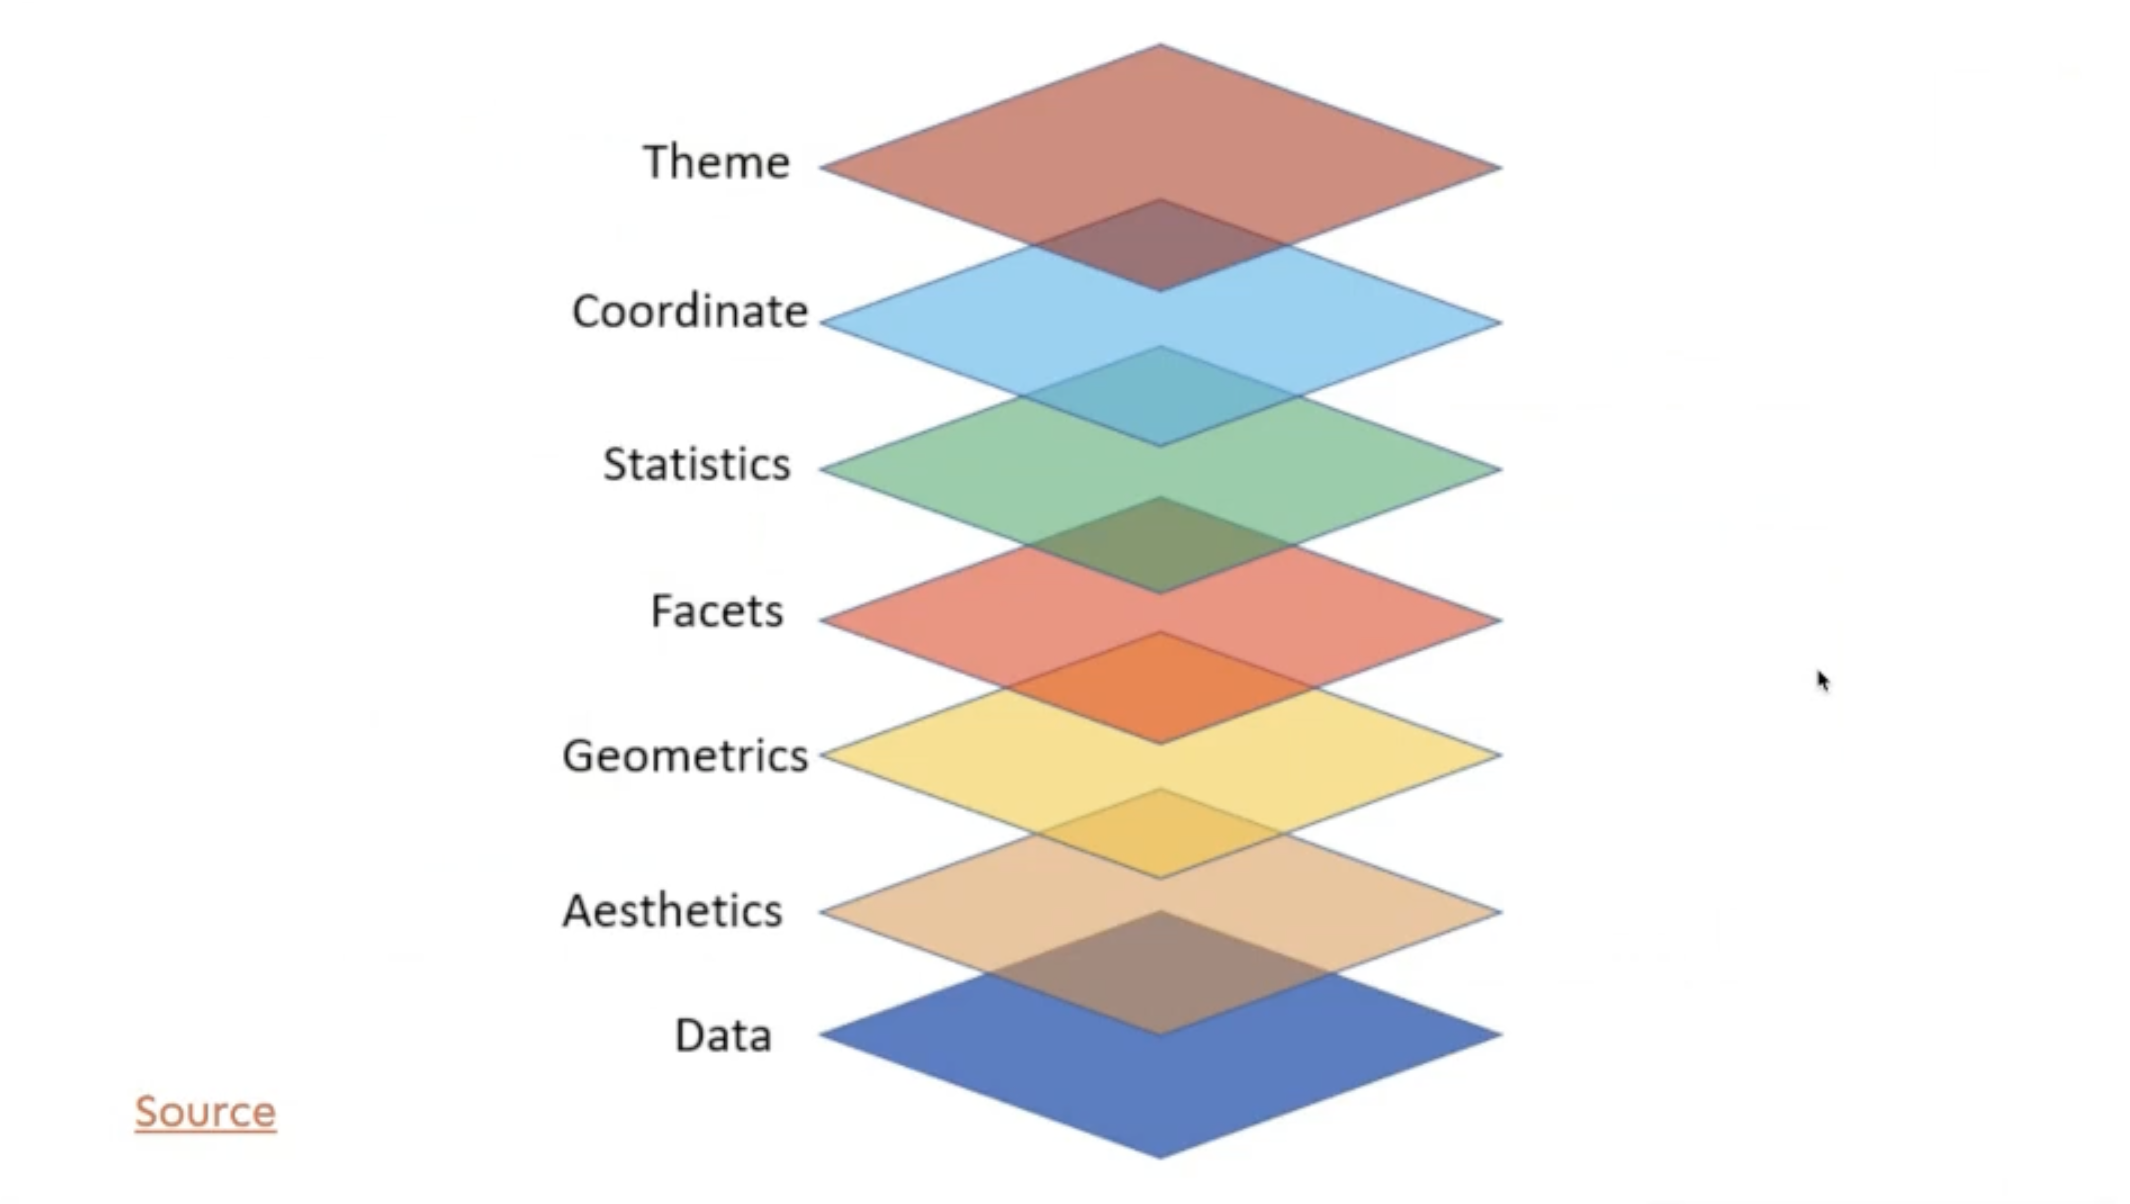
\includegraphics[width=29.58in]{layer_of_data} - Aesthetics: how would
it look like, in terms of what will be on y axis and x axis? What
valuables will be used?

\hypertarget{key-components-of-ggplots2}{%
\subsubsection{Key components of
ggplots2}\label{key-components-of-ggplots2}}

\begin{enumerate}
\def\labelenumi{\arabic{enumi}.}
\tightlist
\item
  data
\item
  aesthetic mapping
\item
  at least one layer of geom function
\end{enumerate}

\begin{Shaded}
\begin{Highlighting}[]
\CommentTok{\# data: call data}
\CommentTok{\# mapping: aesthetic mapping}
\CommentTok{\# geom\_bar: bar as geom function}
\FunctionTok{ggplot}\NormalTok{(}\AttributeTok{data =}\NormalTok{ penguins, }\AttributeTok{mapping =} \FunctionTok{aes}\NormalTok{(}\AttributeTok{x =}\NormalTok{ species)) }\SpecialCharTok{+} \FunctionTok{geom\_bar}\NormalTok{()}
\end{Highlighting}
\end{Shaded}

\includegraphics{Walkthrough_notes_files/figure-latex/unnamed-chunk-18-1.pdf}

\begin{Shaded}
\begin{Highlighting}[]
\CommentTok{\# another example}
\FunctionTok{ggplot}\NormalTok{(}\AttributeTok{data =}\NormalTok{ penguins, }\FunctionTok{aes}\NormalTok{(}\AttributeTok{x =}\NormalTok{ island)) }\SpecialCharTok{+} \FunctionTok{geom\_bar}\NormalTok{()}
\end{Highlighting}
\end{Shaded}

\includegraphics{Walkthrough_notes_files/figure-latex/unnamed-chunk-18-2.pdf}

\hypertarget{how-to-export-plots-to-your-computer}{%
\subsubsection{How to export plots to your
computer}\label{how-to-export-plots-to-your-computer}}

\begin{Shaded}
\begin{Highlighting}[]
\FunctionTok{ggplot}\NormalTok{(}\AttributeTok{data =}\NormalTok{ penguins, }\FunctionTok{aes}\NormalTok{(}\AttributeTok{x =}\NormalTok{ island)) }\SpecialCharTok{+} \FunctionTok{geom\_bar}\NormalTok{()}
\end{Highlighting}
\end{Shaded}

\includegraphics{Walkthrough_notes_files/figure-latex/unnamed-chunk-19-1.pdf}

\begin{Shaded}
\begin{Highlighting}[]
\FunctionTok{ggsave}\NormalTok{(}\StringTok{"peng{-}species.pdf"}\NormalTok{) }\CommentTok{\#also try jpg/jpeg/png}
\end{Highlighting}
\end{Shaded}

\begin{verbatim}
## Saving 6.5 x 4.5 in image
\end{verbatim}

\hypertarget{add-colors-to-bar}{%
\subsubsection{Add colors to bar}\label{add-colors-to-bar}}

\begin{Shaded}
\begin{Highlighting}[]
\FunctionTok{ggplot}\NormalTok{(}\AttributeTok{data =}\NormalTok{ penguins, }\FunctionTok{aes}\NormalTok{(}\AttributeTok{x =}\NormalTok{ island)) }\SpecialCharTok{+} 
  \FunctionTok{geom\_bar}\NormalTok{(}\AttributeTok{fill =} \StringTok{"blue"}\NormalTok{)}
\end{Highlighting}
\end{Shaded}

\includegraphics{Walkthrough_notes_files/figure-latex/unnamed-chunk-20-1.pdf}

\begin{Shaded}
\begin{Highlighting}[]
\CommentTok{\# multiple color}
\CommentTok{\# number of color should = number of factors}
\FunctionTok{ggplot}\NormalTok{(}\AttributeTok{data =}\NormalTok{ penguins, }\FunctionTok{aes}\NormalTok{(}\AttributeTok{x =}\NormalTok{ island)) }\SpecialCharTok{+} 
  \FunctionTok{geom\_bar}\NormalTok{(}\AttributeTok{fill =} \FunctionTok{c}\NormalTok{(}\StringTok{"orange"}\NormalTok{, }\StringTok{"white"}\NormalTok{, }\StringTok{"green"}\NormalTok{))}
\end{Highlighting}
\end{Shaded}

\includegraphics{Walkthrough_notes_files/figure-latex/unnamed-chunk-20-2.pdf}

\hypertarget{add-color-using-palette}{%
\paragraph{Add color using palette}\label{add-color-using-palette}}

\begin{Shaded}
\begin{Highlighting}[]
\CommentTok{\# load packages}
\FunctionTok{library}\NormalTok{(ggplot2)}
\FunctionTok{library}\NormalTok{(RColorBrewer)}
\FunctionTok{library}\NormalTok{(wesanderson)}
\CommentTok{\# Show all options from RColorBrewer}
\FunctionTok{display.brewer.all}\NormalTok{()}
\end{Highlighting}
\end{Shaded}

\includegraphics{Walkthrough_notes_files/figure-latex/ColorPalette-1.pdf}

\begin{Shaded}
\begin{Highlighting}[]
\CommentTok{\# Using RColorBrewer}
\FunctionTok{ggplot}\NormalTok{(}\AttributeTok{data =}\NormalTok{ penguins, }\FunctionTok{aes}\NormalTok{(}\AttributeTok{x =}\NormalTok{ island, }
\CommentTok{\# change                            }
                            \AttributeTok{fill =}\NormalTok{ island)) }\SpecialCharTok{+} 
  \FunctionTok{geom\_bar}\NormalTok{() }\SpecialCharTok{+} 
\CommentTok{\# change 2  }
    \FunctionTok{scale\_fill\_brewer}\NormalTok{(}\AttributeTok{palette =} \StringTok{"Dark2"}\NormalTok{)}
\end{Highlighting}
\end{Shaded}

\includegraphics{Walkthrough_notes_files/figure-latex/unnamed-chunk-21-1.pdf}

\hypertarget{how-to-remove-legends-or-change-its-position}{%
\subsubsection{How to remove legends or change its
position}\label{how-to-remove-legends-or-change-its-position}}

\begin{Shaded}
\begin{Highlighting}[]
\FunctionTok{ggplot}\NormalTok{(}\AttributeTok{data =}\NormalTok{ penguins, }\FunctionTok{aes}\NormalTok{(}\AttributeTok{x =}\NormalTok{ island, }
                            \AttributeTok{fill =}\NormalTok{ island)) }\SpecialCharTok{+} 
  \FunctionTok{geom\_bar}\NormalTok{() }\SpecialCharTok{+} 
    \FunctionTok{scale\_fill\_brewer}\NormalTok{(}\AttributeTok{palette =} \StringTok{"Dark2"}\NormalTok{) }\SpecialCharTok{+}
\CommentTok{\# change}
\FunctionTok{theme}\NormalTok{(}\AttributeTok{legend.position =} \StringTok{"none"}\NormalTok{) }\CommentTok{\# top/bottom/left/right/none}
\end{Highlighting}
\end{Shaded}

\includegraphics{Walkthrough_notes_files/figure-latex/unnamed-chunk-22-1.pdf}

\hypertarget{how-to-plot-title-and-and-axis-titles}{%
\subsubsection{How to plot title and and axis
titles?}\label{how-to-plot-title-and-and-axis-titles}}

\begin{Shaded}
\begin{Highlighting}[]
\FunctionTok{ggplot}\NormalTok{(}\AttributeTok{data =}\NormalTok{ penguins, }\FunctionTok{aes}\NormalTok{(}\AttributeTok{x =}\NormalTok{ island, }
                            \AttributeTok{fill =}\NormalTok{ island)) }\SpecialCharTok{+} 
  \FunctionTok{geom\_bar}\NormalTok{() }\SpecialCharTok{+} 
    \FunctionTok{scale\_fill\_brewer}\NormalTok{(}\AttributeTok{palette =} \StringTok{"Dark2"}\NormalTok{) }\SpecialCharTok{+}
  \FunctionTok{theme}\NormalTok{(}\AttributeTok{legend.position =} \StringTok{"none"}\NormalTok{) }\SpecialCharTok{+}
\CommentTok{\# change}
  \FunctionTok{labs}\NormalTok{(}
    \AttributeTok{title =} \StringTok{"Species of palmer penguins"}\NormalTok{, }
    \AttributeTok{subtitle =} \StringTok{"This data is about penguins"}\NormalTok{, }
    \AttributeTok{x =} \StringTok{"island"}\NormalTok{, }
    \AttributeTok{y =} \StringTok{"Frequency"}
\NormalTok{  )}
\end{Highlighting}
\end{Shaded}

\includegraphics{Walkthrough_notes_files/figure-latex/unnamed-chunk-23-1.pdf}

\hypertarget{how-to-control-size-of-text}{%
\subsubsection{How to control size of
text}\label{how-to-control-size-of-text}}

\begin{Shaded}
\begin{Highlighting}[]
\FunctionTok{ggplot}\NormalTok{(}\AttributeTok{data =}\NormalTok{ penguins, }\FunctionTok{aes}\NormalTok{(}\AttributeTok{x =}\NormalTok{ island, }
                            \AttributeTok{fill =}\NormalTok{ island)) }\SpecialCharTok{+} 
  \FunctionTok{geom\_bar}\NormalTok{() }\SpecialCharTok{+} 
    \FunctionTok{scale\_fill\_brewer}\NormalTok{(}\AttributeTok{palette =} \StringTok{"Dark2"}\NormalTok{) }\SpecialCharTok{+}
  \FunctionTok{theme}\NormalTok{(}\AttributeTok{legend.position =} \StringTok{"none"}\NormalTok{, }
\CommentTok{\# change below        }
        \AttributeTok{text =} \FunctionTok{element\_text}\NormalTok{(}\AttributeTok{size =} \DecValTok{20}\NormalTok{)) }\SpecialCharTok{+}
\CommentTok{\# change above}
  \FunctionTok{labs}\NormalTok{(}
    \AttributeTok{title =} \StringTok{"Species of palmer penguins"}\NormalTok{, }
    \AttributeTok{subtitle =} \StringTok{"This data is about penguins"}\NormalTok{, }
    \AttributeTok{x =} \StringTok{"island"}\NormalTok{, }
    \AttributeTok{y =} \StringTok{"Frequency"}
\NormalTok{  )}
\end{Highlighting}
\end{Shaded}

\includegraphics{Walkthrough_notes_files/figure-latex/unnamed-chunk-24-1.pdf}

\hypertarget{more-ggplot}{%
\subsection{More ggplot}\label{more-ggplot}}

\hypertarget{plot-2-numberic-variables}{%
\subsubsection{plot 2 numberic
variables}\label{plot-2-numberic-variables}}

\begin{Shaded}
\begin{Highlighting}[]
\FunctionTok{ggplot}\NormalTok{(}\AttributeTok{data =}\NormalTok{ penguins, }
       \AttributeTok{mapping =} \FunctionTok{aes}\NormalTok{(}\AttributeTok{x =}\NormalTok{ bill\_length\_mm, }
                     \AttributeTok{y =}\NormalTok{ bill\_depth\_mm, }
                     \AttributeTok{color =}\NormalTok{ species)) }\SpecialCharTok{+} 
  \FunctionTok{geom\_point}\NormalTok{() }\SpecialCharTok{+} 
  \FunctionTok{scale\_fill\_brewer}\NormalTok{(}\AttributeTok{palette =} \StringTok{"Dark2"}\NormalTok{) }\SpecialCharTok{+} 
  \FunctionTok{theme}\NormalTok{(}\AttributeTok{legend.position =} \StringTok{"bottom"}\NormalTok{, }
        \AttributeTok{text =} \FunctionTok{element\_text}\NormalTok{(}\AttributeTok{size =} \DecValTok{20}\NormalTok{)) }\SpecialCharTok{+} 
  \FunctionTok{labs}\NormalTok{(}
    \AttributeTok{title =} \StringTok{"This is a title"}\NormalTok{, }
    \AttributeTok{x =} \StringTok{"Bill Length (mm)"}\NormalTok{, }
    \AttributeTok{y =} \StringTok{"Bill Depth (mm)"}
\NormalTok{  )}
\end{Highlighting}
\end{Shaded}

\begin{verbatim}
## Warning: Removed 2 rows containing missing values (geom_point).
\end{verbatim}

\includegraphics{Walkthrough_notes_files/figure-latex/unnamed-chunk-25-1.pdf}

\hypertarget{add-themes-to-ggplot}{%
\subsubsection{Add themes to ggplot}\label{add-themes-to-ggplot}}

\begin{Shaded}
\begin{Highlighting}[]
\FunctionTok{ggplot}\NormalTok{(}\AttributeTok{data =}\NormalTok{ penguins, }
       \AttributeTok{mapping =} \FunctionTok{aes}\NormalTok{(}\AttributeTok{x =}\NormalTok{ bill\_length\_mm, }
                     \AttributeTok{y =}\NormalTok{ bill\_depth\_mm, }
                     \AttributeTok{color =}\NormalTok{ species)) }\SpecialCharTok{+} 
  \FunctionTok{geom\_point}\NormalTok{() }\SpecialCharTok{+} 
  \FunctionTok{scale\_fill\_brewer}\NormalTok{(}\AttributeTok{palette =} \StringTok{"Dark2"}\NormalTok{) }\SpecialCharTok{+} 
  \FunctionTok{theme}\NormalTok{(}\AttributeTok{legend.position =} \StringTok{"bottom"}\NormalTok{, }
        \AttributeTok{text =} \FunctionTok{element\_text}\NormalTok{(}\AttributeTok{size =} \DecValTok{20}\NormalTok{)) }\SpecialCharTok{+} 
  \FunctionTok{labs}\NormalTok{(}
    \AttributeTok{title =} \StringTok{"This is a title"}\NormalTok{, }
    \AttributeTok{x =} \StringTok{"Bill Length (mm)"}\NormalTok{, }
    \AttributeTok{y =} \StringTok{"Bill Depth (mm)"}
\NormalTok{  ) }\SpecialCharTok{+} 
\CommentTok{\# Change  }
  \FunctionTok{theme\_bw}\NormalTok{()}
\end{Highlighting}
\end{Shaded}

\begin{verbatim}
## Warning: Removed 2 rows containing missing values (geom_point).
\end{verbatim}

\includegraphics{Walkthrough_notes_files/figure-latex/unnamed-chunk-26-1.pdf}

\hypertarget{add-regression-to-plot}{%
\subsubsection{Add regression to plot}\label{add-regression-to-plot}}

\begin{Shaded}
\begin{Highlighting}[]
\FunctionTok{ggplot}\NormalTok{(}\AttributeTok{data =}\NormalTok{ penguins, }
       \AttributeTok{mapping =} \FunctionTok{aes}\NormalTok{(}\AttributeTok{x =}\NormalTok{ bill\_length\_mm, }
                     \AttributeTok{y =}\NormalTok{ bill\_depth\_mm, }
                     \AttributeTok{color =}\NormalTok{ species)) }\SpecialCharTok{+} 
  \FunctionTok{geom\_point}\NormalTok{() }\SpecialCharTok{+} 
  \FunctionTok{scale\_fill\_brewer}\NormalTok{(}\AttributeTok{palette =} \StringTok{"Dark2"}\NormalTok{) }\SpecialCharTok{+} 
  \FunctionTok{theme}\NormalTok{(}\AttributeTok{legend.position =} \StringTok{"bottom"}\NormalTok{, }
        \AttributeTok{text =} \FunctionTok{element\_text}\NormalTok{(}\AttributeTok{size =} \DecValTok{20}\NormalTok{)) }\SpecialCharTok{+} 
  \FunctionTok{labs}\NormalTok{(}
    \AttributeTok{title =} \StringTok{"This is a title"}\NormalTok{, }
    \AttributeTok{x =} \StringTok{"Bill Length (mm)"}\NormalTok{, }
    \AttributeTok{y =} \StringTok{"Bill Depth (mm)"}
\NormalTok{  ) }\SpecialCharTok{+} 
  \FunctionTok{theme\_bw}\NormalTok{() }\SpecialCharTok{+} 
\CommentTok{\# change  }
  \FunctionTok{geom\_smooth}\NormalTok{()}
\end{Highlighting}
\end{Shaded}

\begin{verbatim}
## `geom_smooth()` using method = 'loess' and formula 'y ~ x'
\end{verbatim}

\begin{verbatim}
## Warning: Removed 2 rows containing non-finite values (stat_smooth).
\end{verbatim}

\begin{verbatim}
## Warning: Removed 2 rows containing missing values (geom_point).
\end{verbatim}

\includegraphics{Walkthrough_notes_files/figure-latex/unnamed-chunk-27-1.pdf}

\hypertarget{session-4-data-wrangling-with-dplyr}{%
\section{Session 4 Data Wrangling with
dplyr}\label{session-4-data-wrangling-with-dplyr}}

Data wrangling means ``Data exploration and manipulation''. - dplyr:
grammar of data manipulation - important functions:

\begin{enumerate}
\def\labelenumi{\arabic{enumi}.}
\tightlist
\item
  filter()
\item
  select()
\item
  mutate()
\item
  arrange()
\item
  summarise()
\end{enumerate}

\begin{Shaded}
\begin{Highlighting}[]
\FunctionTok{library}\NormalTok{(palmerpenguins)}
\FunctionTok{library}\NormalTok{(dplyr)}
\end{Highlighting}
\end{Shaded}

\hypertarget{filter-pick-only-gentoo-penguins}{%
\subsubsection{filter(): pick only Gentoo
penguins}\label{filter-pick-only-gentoo-penguins}}

\begin{Shaded}
\begin{Highlighting}[]
\NormalTok{penguins }\SpecialCharTok{\%\textgreater{}\%} 
  \FunctionTok{filter}\NormalTok{(species }\SpecialCharTok{==} \StringTok{\textquotesingle{}Gentoo\textquotesingle{}}\NormalTok{)}
\end{Highlighting}
\end{Shaded}

\begin{verbatim}
## # A tibble: 124 x 8
##    species island bill_length_mm bill_depth_mm flipper_length_mm body_mass_g
##    <fct>   <fct>           <dbl>         <dbl>             <int>       <int>
##  1 Gentoo  Biscoe           46.1          13.2               211        4500
##  2 Gentoo  Biscoe           50            16.3               230        5700
##  3 Gentoo  Biscoe           48.7          14.1               210        4450
##  4 Gentoo  Biscoe           50            15.2               218        5700
##  5 Gentoo  Biscoe           47.6          14.5               215        5400
##  6 Gentoo  Biscoe           46.5          13.5               210        4550
##  7 Gentoo  Biscoe           45.4          14.6               211        4800
##  8 Gentoo  Biscoe           46.7          15.3               219        5200
##  9 Gentoo  Biscoe           43.3          13.4               209        4400
## 10 Gentoo  Biscoe           46.8          15.4               215        5150
## # ... with 114 more rows, and 2 more variables: sex <fct>, year <int>
\end{verbatim}

\begin{Shaded}
\begin{Highlighting}[]
\NormalTok{penguins }\SpecialCharTok{\%\textgreater{}\%} 
  \FunctionTok{filter}\NormalTok{(species }\SpecialCharTok{==} \StringTok{\textquotesingle{}Gentoo\textquotesingle{}}\NormalTok{) }\SpecialCharTok{\%\textgreater{}\%} 
  \FunctionTok{summary}\NormalTok{() }\SpecialCharTok{\%\textgreater{}\%} 
\NormalTok{  kableExtra}\SpecialCharTok{::}\FunctionTok{kable}\NormalTok{() }\SpecialCharTok{\%\textgreater{}\%} 
  \FunctionTok{kable\_styling}\NormalTok{()}
\end{Highlighting}
\end{Shaded}

\begin{table}
\centering
\begin{tabular}{l|l|l|l|l|l|l|l|l}
\hline
  &      species &       island & bill\_length\_mm & bill\_depth\_mm & flipper\_length\_mm &  body\_mass\_g &     sex &      year\\
\hline
 & Adelie   :  0 & Biscoe   :124 & Min.   :40.90 & Min.   :13.10 & Min.   :203.0 & Min.   :3950 & female:58 & Min.   :2007\\
\hline
 & Chinstrap:  0 & Dream    :  0 & 1st Qu.:45.30 & 1st Qu.:14.20 & 1st Qu.:212.0 & 1st Qu.:4700 & male  :61 & 1st Qu.:2007\\
\hline
 & Gentoo   :124 & Torgersen:  0 & Median :47.30 & Median :15.00 & Median :216.0 & Median :5000 & NA's  : 5 & Median :2008\\
\hline
 & NA & NA & Mean   :47.50 & Mean   :14.98 & Mean   :217.2 & Mean   :5076 & NA & Mean   :2008\\
\hline
 & NA & NA & 3rd Qu.:49.55 & 3rd Qu.:15.70 & 3rd Qu.:221.0 & 3rd Qu.:5500 & NA & 3rd Qu.:2009\\
\hline
 & NA & NA & Max.   :59.60 & Max.   :17.30 & Max.   :231.0 & Max.   :6300 & NA & Max.   :2009\\
\hline
 & NA & NA & NA's   :1 & NA's   :1 & NA's   :1 & NA's   :1 & NA & NA\\
\hline
\end{tabular}
\end{table}

\hypertarget{more-filter}{%
\subsubsection{More filter():}\label{more-filter}}

\hypertarget{section}{%
\paragraph{1}\label{section}}

\begin{Shaded}
\begin{Highlighting}[]
\NormalTok{penguins }\SpecialCharTok{\%\textgreater{}\%} 
  \FunctionTok{filter}\NormalTok{(bill\_length\_mm }\SpecialCharTok{\textgreater{}} \StringTok{\textquotesingle{}43\textquotesingle{}}\NormalTok{)}
\end{Highlighting}
\end{Shaded}

\begin{verbatim}
## # A tibble: 188 x 8
##    species island    bill_length_mm bill_depth_mm flipper_length_mm body_mass_g
##    <fct>   <fct>              <dbl>         <dbl>             <int>       <int>
##  1 Adelie  Torgersen           46            21.5               194        4200
##  2 Adelie  Dream               44.1          19.7               196        4400
##  3 Adelie  Torgersen           45.8          18.9               197        4150
##  4 Adelie  Dream               43.2          18.5               192        4100
##  5 Adelie  Biscoe              43.2          19                 197        4775
##  6 Adelie  Biscoe              45.6          20.3               191        4600
##  7 Adelie  Torgersen           44.1          18                 210        4000
##  8 Adelie  Torgersen           43.1          19.2               197        3500
##  9 Gentoo  Biscoe              46.1          13.2               211        4500
## 10 Gentoo  Biscoe              50            16.3               230        5700
## # ... with 178 more rows, and 2 more variables: sex <fct>, year <int>
\end{verbatim}

\hypertarget{section-1}{%
\paragraph{2}\label{section-1}}

\begin{Shaded}
\begin{Highlighting}[]
\NormalTok{penguins }\SpecialCharTok{\%\textgreater{}\%} 
  \FunctionTok{filter}\NormalTok{(species }\SpecialCharTok{==} \StringTok{\textquotesingle{}Gentoo\textquotesingle{}}\NormalTok{, }
\NormalTok{         bill\_length\_mm }\SpecialCharTok{\textgreater{}} \StringTok{\textquotesingle{}55\textquotesingle{}}\NormalTok{)}
\end{Highlighting}
\end{Shaded}

\begin{verbatim}
## # A tibble: 3 x 8
##   species island bill_length_mm bill_depth_mm flipper_length_~ body_mass_g sex  
##   <fct>   <fct>           <dbl>         <dbl>            <int>       <int> <fct>
## 1 Gentoo  Biscoe           59.6            17              230        6050 male 
## 2 Gentoo  Biscoe           55.9            17              228        5600 male 
## 3 Gentoo  Biscoe           55.1            16              230        5850 male 
## # ... with 1 more variable: year <int>
\end{verbatim}

\hypertarget{export-data-file-to-computer}{%
\subsubsection{Export data file to
computer}\label{export-data-file-to-computer}}

\begin{Shaded}
\begin{Highlighting}[]
\NormalTok{penguins }\SpecialCharTok{\%\textgreater{}\%} 
  \FunctionTok{filter}\NormalTok{(species }\SpecialCharTok{==} \StringTok{\textquotesingle{}Gentoo\textquotesingle{}}\NormalTok{) }\SpecialCharTok{\%\textgreater{}\%} 
  \FunctionTok{write.csv}\NormalTok{(}\StringTok{\textquotesingle{}gentoo{-}penguins.csv\textquotesingle{}}\NormalTok{)}
\CommentTok{\# a new csv file is saved into the project folder}
\end{Highlighting}
\end{Shaded}

\hypertarget{pipe}{%
\subsubsection{Pipe \%\textgreater\%}\label{pipe}}

\begin{itemize}
\tightlist
\item
  control + shift + m
\item
  sequencing multiple operations
\end{itemize}

\hypertarget{comparison-relational-operators}{%
\subsubsection{Comparison: Relational
Operators}\label{comparison-relational-operators}}

\begin{itemize}
\tightlist
\item
  x \textgreater{} y
\item
  x \textless{} y
\item
  x \textgreater= y
\item
  x \textless= y
\item
  x == y (equal)
\item
  x != y (not equal)
\end{itemize}

\hypertarget{how-to-have-only-top-or-bottom-rows-from-data}{%
\subsubsection{How to have only top or bottom rows from
data?}\label{how-to-have-only-top-or-bottom-rows-from-data}}

\begin{Shaded}
\begin{Highlighting}[]
\NormalTok{penguins }\SpecialCharTok{\%\textgreater{}\%} 
  \FunctionTok{filter}\NormalTok{(bill\_length\_mm }\SpecialCharTok{\textgreater{}} \StringTok{\textquotesingle{}43\textquotesingle{}}\NormalTok{) }\SpecialCharTok{\%\textgreater{}\%} 
\CommentTok{\# head to only show first 6 rows}
  \FunctionTok{head}\NormalTok{()}
\end{Highlighting}
\end{Shaded}

\begin{verbatim}
## # A tibble: 6 x 8
##   species island bill_length_mm bill_depth_mm flipper_length_~ body_mass_g sex  
##   <fct>   <fct>           <dbl>         <dbl>            <int>       <int> <fct>
## 1 Adelie  Torge~           46            21.5              194        4200 male 
## 2 Adelie  Dream            44.1          19.7              196        4400 male 
## 3 Adelie  Torge~           45.8          18.9              197        4150 male 
## 4 Adelie  Dream            43.2          18.5              192        4100 male 
## 5 Adelie  Biscoe           43.2          19                197        4775 male 
## 6 Adelie  Biscoe           45.6          20.3              191        4600 male 
## # ... with 1 more variable: year <int>
\end{verbatim}

\begin{Shaded}
\begin{Highlighting}[]
\NormalTok{penguins }\SpecialCharTok{\%\textgreater{}\%} 
  \FunctionTok{filter}\NormalTok{(bill\_length\_mm }\SpecialCharTok{\textgreater{}} \StringTok{\textquotesingle{}43\textquotesingle{}}\NormalTok{) }\SpecialCharTok{\%\textgreater{}\%} 
\CommentTok{\# tail to only show lowest 6 rows  }
\CommentTok{\# use tail(number) [e.g. tail(3)] to restrict the number of rows shown}
  \FunctionTok{tail}\NormalTok{()}
\end{Highlighting}
\end{Shaded}

\begin{verbatim}
## # A tibble: 6 x 8
##   species island bill_length_mm bill_depth_mm flipper_length_~ body_mass_g sex  
##   <fct>   <fct>           <dbl>         <dbl>            <int>       <int> <fct>
## 1 Chinst~ Dream            45.7          17                195        3650 fema~
## 2 Chinst~ Dream            55.8          19.8              207        4000 male 
## 3 Chinst~ Dream            43.5          18.1              202        3400 fema~
## 4 Chinst~ Dream            49.6          18.2              193        3775 male 
## 5 Chinst~ Dream            50.8          19                210        4100 male 
## 6 Chinst~ Dream            50.2          18.7              198        3775 fema~
## # ... with 1 more variable: year <int>
\end{verbatim}

\begin{Shaded}
\begin{Highlighting}[]
\NormalTok{penguins }\SpecialCharTok{\%\textgreater{}\%} 
  \FunctionTok{filter}\NormalTok{(species }\SpecialCharTok{==} \StringTok{"Chinstrap"}\NormalTok{, }
\NormalTok{         bill\_length\_mm }\SpecialCharTok{\textgreater{}} \DecValTok{45}\NormalTok{, }
\NormalTok{         body\_mass\_g }\SpecialCharTok{\textgreater{}} \DecValTok{4000}\NormalTok{) }
\end{Highlighting}
\end{Shaded}

\begin{verbatim}
## # A tibble: 15 x 8
##    species   island bill_length_mm bill_depth_mm flipper_length_mm body_mass_g
##    <fct>     <fct>           <dbl>         <dbl>             <int>       <int>
##  1 Chinstrap Dream            46            18.9               195        4150
##  2 Chinstrap Dream            52            18.1               201        4050
##  3 Chinstrap Dream            50.5          19.6               201        4050
##  4 Chinstrap Dream            49.2          18.2               195        4400
##  5 Chinstrap Dream            52            19                 197        4150
##  6 Chinstrap Dream            52.8          20                 205        4550
##  7 Chinstrap Dream            54.2          20.8               201        4300
##  8 Chinstrap Dream            51            18.8               203        4100
##  9 Chinstrap Dream            52            20.7               210        4800
## 10 Chinstrap Dream            53.5          19.9               205        4500
## 11 Chinstrap Dream            50.8          18.5               201        4450
## 12 Chinstrap Dream            49            19.6               212        4300
## 13 Chinstrap Dream            50.7          19.7               203        4050
## 14 Chinstrap Dream            49.3          19.9               203        4050
## 15 Chinstrap Dream            50.8          19                 210        4100
## # ... with 2 more variables: sex <fct>, year <int>
\end{verbatim}

\hypertarget{select}{%
\subsubsection{select()}\label{select}}

\begin{Shaded}
\begin{Highlighting}[]
\NormalTok{penguins }\SpecialCharTok{\%\textgreater{}\%} 
  \FunctionTok{select}\NormalTok{(species)}
\end{Highlighting}
\end{Shaded}

\begin{verbatim}
## # A tibble: 344 x 1
##    species
##    <fct>  
##  1 Adelie 
##  2 Adelie 
##  3 Adelie 
##  4 Adelie 
##  5 Adelie 
##  6 Adelie 
##  7 Adelie 
##  8 Adelie 
##  9 Adelie 
## 10 Adelie 
## # ... with 334 more rows
\end{verbatim}

\begin{Shaded}
\begin{Highlighting}[]
\CommentTok{\# Only variables from species to bill\_length\_mm}
\NormalTok{penguins }\SpecialCharTok{\%\textgreater{}\%} 
  \FunctionTok{select}\NormalTok{(species }\SpecialCharTok{:}\NormalTok{ bill\_length\_mm)}
\end{Highlighting}
\end{Shaded}

\begin{verbatim}
## # A tibble: 344 x 3
##    species island    bill_length_mm
##    <fct>   <fct>              <dbl>
##  1 Adelie  Torgersen           39.1
##  2 Adelie  Torgersen           39.5
##  3 Adelie  Torgersen           40.3
##  4 Adelie  Torgersen           NA  
##  5 Adelie  Torgersen           36.7
##  6 Adelie  Torgersen           39.3
##  7 Adelie  Torgersen           38.9
##  8 Adelie  Torgersen           39.2
##  9 Adelie  Torgersen           34.1
## 10 Adelie  Torgersen           42  
## # ... with 334 more rows
\end{verbatim}

\begin{Shaded}
\begin{Highlighting}[]
\CommentTok{\# You can also use the order of range to select variables}
\NormalTok{penguins }\SpecialCharTok{\%\textgreater{}\%} 
  \FunctionTok{select}\NormalTok{(}\DecValTok{4}\SpecialCharTok{:}\DecValTok{8}\NormalTok{)}
\end{Highlighting}
\end{Shaded}

\begin{verbatim}
## # A tibble: 344 x 5
##    bill_depth_mm flipper_length_mm body_mass_g sex     year
##            <dbl>             <int>       <int> <fct>  <int>
##  1          18.7               181        3750 male    2007
##  2          17.4               186        3800 female  2007
##  3          18                 195        3250 female  2007
##  4          NA                  NA          NA <NA>    2007
##  5          19.3               193        3450 female  2007
##  6          20.6               190        3650 male    2007
##  7          17.8               181        3625 female  2007
##  8          19.6               195        4675 male    2007
##  9          18.1               193        3475 <NA>    2007
## 10          20.2               190        4250 <NA>    2007
## # ... with 334 more rows
\end{verbatim}

\begin{Shaded}
\begin{Highlighting}[]
\CommentTok{\# For specific variables}
\NormalTok{penguins }\SpecialCharTok{\%\textgreater{}\%} 
  \FunctionTok{select}\NormalTok{(bill\_depth\_mm, body\_mass\_g)}
\end{Highlighting}
\end{Shaded}

\begin{verbatim}
## # A tibble: 344 x 2
##    bill_depth_mm body_mass_g
##            <dbl>       <int>
##  1          18.7        3750
##  2          17.4        3800
##  3          18          3250
##  4          NA            NA
##  5          19.3        3450
##  6          20.6        3650
##  7          17.8        3625
##  8          19.6        4675
##  9          18.1        3475
## 10          20.2        4250
## # ... with 334 more rows
\end{verbatim}

\begin{Shaded}
\begin{Highlighting}[]
\CommentTok{\# Select except some specific variables using {-}c()}
\NormalTok{penguins }\SpecialCharTok{\%\textgreater{}\%} 
  \FunctionTok{select}\NormalTok{(}\SpecialCharTok{{-}}\FunctionTok{c}\NormalTok{(bill\_depth\_mm, year))}
\end{Highlighting}
\end{Shaded}

\begin{verbatim}
## # A tibble: 344 x 6
##    species island    bill_length_mm flipper_length_mm body_mass_g sex   
##    <fct>   <fct>              <dbl>             <int>       <int> <fct> 
##  1 Adelie  Torgersen           39.1               181        3750 male  
##  2 Adelie  Torgersen           39.5               186        3800 female
##  3 Adelie  Torgersen           40.3               195        3250 female
##  4 Adelie  Torgersen           NA                  NA          NA <NA>  
##  5 Adelie  Torgersen           36.7               193        3450 female
##  6 Adelie  Torgersen           39.3               190        3650 male  
##  7 Adelie  Torgersen           38.9               181        3625 female
##  8 Adelie  Torgersen           39.2               195        4675 male  
##  9 Adelie  Torgersen           34.1               193        3475 <NA>  
## 10 Adelie  Torgersen           42                 190        4250 <NA>  
## # ... with 334 more rows
\end{verbatim}

\hypertarget{mutate-add-new-variables-that-are-functions-of-existing-variables}{%
\subsubsection{mutate(): Add new variables that are functions of
existing
variables}\label{mutate-add-new-variables-that-are-functions-of-existing-variables}}

\begin{Shaded}
\begin{Highlighting}[]
\CommentTok{\# Covert penguin body mass from grams to kilograms}
\NormalTok{penguins }\SpecialCharTok{\%\textgreater{}\%} 
  \FunctionTok{mutate}\NormalTok{(}\AttributeTok{body\_mass\_kg =}\NormalTok{ body\_mass\_g }\SpecialCharTok{/} \DecValTok{1000}\NormalTok{)}
\end{Highlighting}
\end{Shaded}

\begin{verbatim}
## # A tibble: 344 x 9
##    species island    bill_length_mm bill_depth_mm flipper_length_mm body_mass_g
##    <fct>   <fct>              <dbl>         <dbl>             <int>       <int>
##  1 Adelie  Torgersen           39.1          18.7               181        3750
##  2 Adelie  Torgersen           39.5          17.4               186        3800
##  3 Adelie  Torgersen           40.3          18                 195        3250
##  4 Adelie  Torgersen           NA            NA                  NA          NA
##  5 Adelie  Torgersen           36.7          19.3               193        3450
##  6 Adelie  Torgersen           39.3          20.6               190        3650
##  7 Adelie  Torgersen           38.9          17.8               181        3625
##  8 Adelie  Torgersen           39.2          19.6               195        4675
##  9 Adelie  Torgersen           34.1          18.1               193        3475
## 10 Adelie  Torgersen           42            20.2               190        4250
## # ... with 334 more rows, and 3 more variables: sex <fct>, year <int>,
## #   body_mass_kg <dbl>
\end{verbatim}

\begin{Shaded}
\begin{Highlighting}[]
\CommentTok{\# If you just want the 2 related variables}
\NormalTok{penguins }\SpecialCharTok{\%\textgreater{}\%} 
  \FunctionTok{select}\NormalTok{(body\_mass\_g) }\SpecialCharTok{\%\textgreater{}\%} 
  \FunctionTok{mutate}\NormalTok{(}\AttributeTok{body\_mass\_kg =}\NormalTok{ body\_mass\_g }\SpecialCharTok{/} \DecValTok{1000}\NormalTok{)}
\end{Highlighting}
\end{Shaded}

\begin{verbatim}
## # A tibble: 344 x 2
##    body_mass_g body_mass_kg
##          <int>        <dbl>
##  1        3750         3.75
##  2        3800         3.8 
##  3        3250         3.25
##  4          NA        NA   
##  5        3450         3.45
##  6        3650         3.65
##  7        3625         3.62
##  8        4675         4.68
##  9        3475         3.48
## 10        4250         4.25
## # ... with 334 more rows
\end{verbatim}

\begin{Shaded}
\begin{Highlighting}[]
\CommentTok{\# Add 2 variables at the same time}
\NormalTok{penguins }\SpecialCharTok{\%\textgreater{}\%} 
  \FunctionTok{mutate}\NormalTok{(}\AttributeTok{body\_mass\_kg =}\NormalTok{ body\_mass\_g }\SpecialCharTok{/} \DecValTok{1000}\NormalTok{, }
         \AttributeTok{bill =}\NormalTok{ bill\_length\_mm }\SpecialCharTok{*}\NormalTok{ bill\_depth\_mm)}
\end{Highlighting}
\end{Shaded}

\begin{verbatim}
## # A tibble: 344 x 10
##    species island    bill_length_mm bill_depth_mm flipper_length_mm body_mass_g
##    <fct>   <fct>              <dbl>         <dbl>             <int>       <int>
##  1 Adelie  Torgersen           39.1          18.7               181        3750
##  2 Adelie  Torgersen           39.5          17.4               186        3800
##  3 Adelie  Torgersen           40.3          18                 195        3250
##  4 Adelie  Torgersen           NA            NA                  NA          NA
##  5 Adelie  Torgersen           36.7          19.3               193        3450
##  6 Adelie  Torgersen           39.3          20.6               190        3650
##  7 Adelie  Torgersen           38.9          17.8               181        3625
##  8 Adelie  Torgersen           39.2          19.6               195        4675
##  9 Adelie  Torgersen           34.1          18.1               193        3475
## 10 Adelie  Torgersen           42            20.2               190        4250
## # ... with 334 more rows, and 4 more variables: sex <fct>, year <int>,
## #   body_mass_kg <dbl>, bill <dbl>
\end{verbatim}

\begin{Shaded}
\begin{Highlighting}[]
\CommentTok{\# Show only the new variables}
\NormalTok{penguins }\SpecialCharTok{\%\textgreater{}\%} 
  \FunctionTok{mutate}\NormalTok{(}\AttributeTok{body\_mass\_kg =}\NormalTok{ body\_mass\_g }\SpecialCharTok{/} \DecValTok{1000}\NormalTok{, }
         \AttributeTok{bill =}\NormalTok{ bill\_length\_mm }\SpecialCharTok{*}\NormalTok{ bill\_depth\_mm) }\SpecialCharTok{\%\textgreater{}\%} 
  \FunctionTok{select}\NormalTok{(body\_mass\_kg, }
\NormalTok{         bill)}
\end{Highlighting}
\end{Shaded}

\begin{verbatim}
## # A tibble: 344 x 2
##    body_mass_kg  bill
##           <dbl> <dbl>
##  1         3.75  731.
##  2         3.8   687.
##  3         3.25  725.
##  4        NA      NA 
##  5         3.45  708.
##  6         3.65  810.
##  7         3.62  692.
##  8         4.68  768.
##  9         3.48  617.
## 10         4.25  848.
## # ... with 334 more rows
\end{verbatim}

\hypertarget{arrange-changes-the-order-of-the-rows}{%
\subsubsection{arrange(): Changes the order of the
rows}\label{arrange-changes-the-order-of-the-rows}}

\begin{Shaded}
\begin{Highlighting}[]
\CommentTok{\# Arrange the data by ascending order of bill length}
\NormalTok{penguins }\SpecialCharTok{\%\textgreater{}\%} 
  \FunctionTok{arrange}\NormalTok{(bill\_length\_mm)}
\end{Highlighting}
\end{Shaded}

\begin{verbatim}
## # A tibble: 344 x 8
##    species island    bill_length_mm bill_depth_mm flipper_length_mm body_mass_g
##    <fct>   <fct>              <dbl>         <dbl>             <int>       <int>
##  1 Adelie  Dream               32.1          15.5               188        3050
##  2 Adelie  Dream               33.1          16.1               178        2900
##  3 Adelie  Torgersen           33.5          19                 190        3600
##  4 Adelie  Dream               34            17.1               185        3400
##  5 Adelie  Torgersen           34.1          18.1               193        3475
##  6 Adelie  Torgersen           34.4          18.4               184        3325
##  7 Adelie  Biscoe              34.5          18.1               187        2900
##  8 Adelie  Torgersen           34.6          21.1               198        4400
##  9 Adelie  Torgersen           34.6          17.2               189        3200
## 10 Adelie  Biscoe              35            17.9               190        3450
## # ... with 334 more rows, and 2 more variables: sex <fct>, year <int>
\end{verbatim}

\begin{Shaded}
\begin{Highlighting}[]
\CommentTok{\# In desc order}
\NormalTok{penguins }\SpecialCharTok{\%\textgreater{}\%} 
  \FunctionTok{arrange}\NormalTok{(}\FunctionTok{desc}\NormalTok{(bill\_length\_mm))}
\end{Highlighting}
\end{Shaded}

\begin{verbatim}
## # A tibble: 344 x 8
##    species   island bill_length_mm bill_depth_mm flipper_length_mm body_mass_g
##    <fct>     <fct>           <dbl>         <dbl>             <int>       <int>
##  1 Gentoo    Biscoe           59.6          17                 230        6050
##  2 Chinstrap Dream            58            17.8               181        3700
##  3 Gentoo    Biscoe           55.9          17                 228        5600
##  4 Chinstrap Dream            55.8          19.8               207        4000
##  5 Gentoo    Biscoe           55.1          16                 230        5850
##  6 Gentoo    Biscoe           54.3          15.7               231        5650
##  7 Chinstrap Dream            54.2          20.8               201        4300
##  8 Chinstrap Dream            53.5          19.9               205        4500
##  9 Gentoo    Biscoe           53.4          15.8               219        5500
## 10 Chinstrap Dream            52.8          20                 205        4550
## # ... with 334 more rows, and 2 more variables: sex <fct>, year <int>
\end{verbatim}

\begin{Shaded}
\begin{Highlighting}[]
\CommentTok{\# Non{-}numeric variables work too}
\NormalTok{penguins }\SpecialCharTok{\%\textgreater{}\%} 
  \FunctionTok{arrange}\NormalTok{(species)}
\end{Highlighting}
\end{Shaded}

\begin{verbatim}
## # A tibble: 344 x 8
##    species island    bill_length_mm bill_depth_mm flipper_length_mm body_mass_g
##    <fct>   <fct>              <dbl>         <dbl>             <int>       <int>
##  1 Adelie  Torgersen           39.1          18.7               181        3750
##  2 Adelie  Torgersen           39.5          17.4               186        3800
##  3 Adelie  Torgersen           40.3          18                 195        3250
##  4 Adelie  Torgersen           NA            NA                  NA          NA
##  5 Adelie  Torgersen           36.7          19.3               193        3450
##  6 Adelie  Torgersen           39.3          20.6               190        3650
##  7 Adelie  Torgersen           38.9          17.8               181        3625
##  8 Adelie  Torgersen           39.2          19.6               195        4675
##  9 Adelie  Torgersen           34.1          18.1               193        3475
## 10 Adelie  Torgersen           42            20.2               190        4250
## # ... with 334 more rows, and 2 more variables: sex <fct>, year <int>
\end{verbatim}

\hypertarget{summarise-choose-rows-based-on-column-values}{%
\subsubsection{summarise(): choose rows based on column
values}\label{summarise-choose-rows-based-on-column-values}}

\begin{Shaded}
\begin{Highlighting}[]
\CommentTok{\# Mean bill length of all penguins}
\NormalTok{penguins }\SpecialCharTok{\%\textgreater{}\%} 
\CommentTok{\# drop\_na to avoid n/a cells because they do not work with statistics calculations  }
\NormalTok{  drop\_na }\SpecialCharTok{\%\textgreater{}\%} 
  \FunctionTok{summarise}\NormalTok{(}\AttributeTok{mean\_bill\_length\_mm =} \FunctionTok{mean}\NormalTok{(bill\_length\_mm))}
\end{Highlighting}
\end{Shaded}

\begin{verbatim}
## # A tibble: 1 x 1
##   mean_bill_length_mm
##                 <dbl>
## 1                44.0
\end{verbatim}

\begin{Shaded}
\begin{Highlighting}[]
\CommentTok{\# Find species{-}wise mean bill length of all penguins with group\_by()}
\NormalTok{penguins }\SpecialCharTok{\%\textgreater{}\%} 
\NormalTok{  drop\_na }\SpecialCharTok{\%\textgreater{}\%} 
  \FunctionTok{group\_by}\NormalTok{(species) }\SpecialCharTok{\%\textgreater{}\%} 
  \FunctionTok{summarise}\NormalTok{(}\AttributeTok{mean\_bill\_length\_mm =} \FunctionTok{mean}\NormalTok{(bill\_length\_mm))}
\end{Highlighting}
\end{Shaded}

\begin{verbatim}
## # A tibble: 3 x 2
##   species   mean_bill_length_mm
##   <fct>                   <dbl>
## 1 Adelie                   38.8
## 2 Chinstrap                48.8
## 3 Gentoo                   47.6
\end{verbatim}

\begin{Shaded}
\begin{Highlighting}[]
\CommentTok{\# Find species{-}wise mean bill length of all penguins and total number of penguins in each species}
\NormalTok{penguins }\SpecialCharTok{\%\textgreater{}\%} 
\NormalTok{  drop\_na }\SpecialCharTok{\%\textgreater{}\%} 
  \FunctionTok{group\_by}\NormalTok{(species) }\SpecialCharTok{\%\textgreater{}\%} 
  \FunctionTok{summarise}\NormalTok{(}\AttributeTok{mean\_bill\_length\_mm =} \FunctionTok{mean}\NormalTok{(bill\_length\_mm), }
\CommentTok{\# n() calculate how many elements are in the variable        }
\CommentTok{\# Sometimes you should use count() instead}
\CommentTok{\# n() only work for specific group size (e.g. within mutate() or summarise())}
            \AttributeTok{n =} \FunctionTok{n}\NormalTok{())}
\end{Highlighting}
\end{Shaded}

\begin{verbatim}
## # A tibble: 3 x 3
##   species   mean_bill_length_mm     n
##   <fct>                   <dbl> <int>
## 1 Adelie                   38.8   146
## 2 Chinstrap                48.8    68
## 3 Gentoo                   47.6   119
\end{verbatim}

\end{document}
